%\chapter{Preliminaries}
\chapter{実験1 -色情報による光沢感変化-}

    \section{目的}
        実験1では,輝度は同一であるが色度のみが異なる刺激に対して知覚される光沢感を測定する.
        色度ごとの光沢感を定量化することで,光沢感に色度情報が寄与しているかどうかを明らかにすることを目的とする.

        \subsection{仮説}
            第1章で述べたとおり,物体の表面の輝度成分が光沢感知覚に寄与していることは既知である.
            しかし,輝度が変わると当然知覚的な明るさも変わるため,光沢感に寄与しているのが知覚的な明るさ感なのか輝度情報そのものなのかについては明らかになっていない.
            輝度と知覚的な明るさ感が分離される現象としてHelmholtz-Kohlrausch効果(以下H-K効果)が知られている.
            これは,同一の輝度を有する色でも彩度が高いほど明るく感じられ,特に青・紫・赤紫・赤などの色相を有する色がより明るく見えるという効果である.
            このように,有彩色刺激を採用しH-K効果を利用することにより,輝度の明るさを分離することが可能となる.

            本研究で検証する仮説は,拡散反射成分と鏡面反射成分の知覚的な明るさ感のコントラストが主に光沢感に寄与しているというものである.
            従来の研究から,拡散反射成分と鏡面反射成分の輝度コントラストが知覚的光沢感に強く寄与することが明らかになっている.\cite{Hunter}

            本実験で検証するのは,この輝度コントラストに起因するものであったという可能性に関する仮説となる.ここで,鏡面反射成分と拡散反射成分の色度情報を利用して明るさ感のみを変化させれば,輝度の効果と明るさの効果を検証できるはずである.
            反射成分のうち,拡散反射成分は鏡面反射成分に比べて多くの場合には低輝度である.
            そこで反射成分を拡散反射成分と鏡面反射成分に分け,拡散反射成分のみに輝度を変えずに色度を変化させ有彩色を付与する処理を行う.
            このとき,もし上述の仮説が正しいとすれば,H-K効果による明るさ感の増幅が顕著な色度では,拡散反射成分の明るさ感がH-K効果により向上することに起因し,他色度に比べて相対的に明るさ感のコントラストが大きく減少するため,光沢感が小さくなるはずである.
            一方で,コントロール刺激として拡散反射成分と鏡面反射成分の両方に輝度を変えずに色度を変化させた刺激を用意する.
            この刺激は拡散反射成分と鏡面反射成分の両方の明るさ感がH-K効果により向上するため,明るさのコントラストは相対的に小さい.
            明るさ感のコントラストが光沢感知覚に寄与しているならば,この2種類の刺激に対する応答の傾向は異なるはずである.

    \section{実験方法}
        \subsection{被験者}
            本実験は20代男性7人に対して行われた.
            全被験者の視力または矯正視力は正常であり,かつ石原式色覚異常検査表により色覚が正常であることが確認されていた.

        \subsection{実験環境}

            \begin{figure}[h]
                \centering
                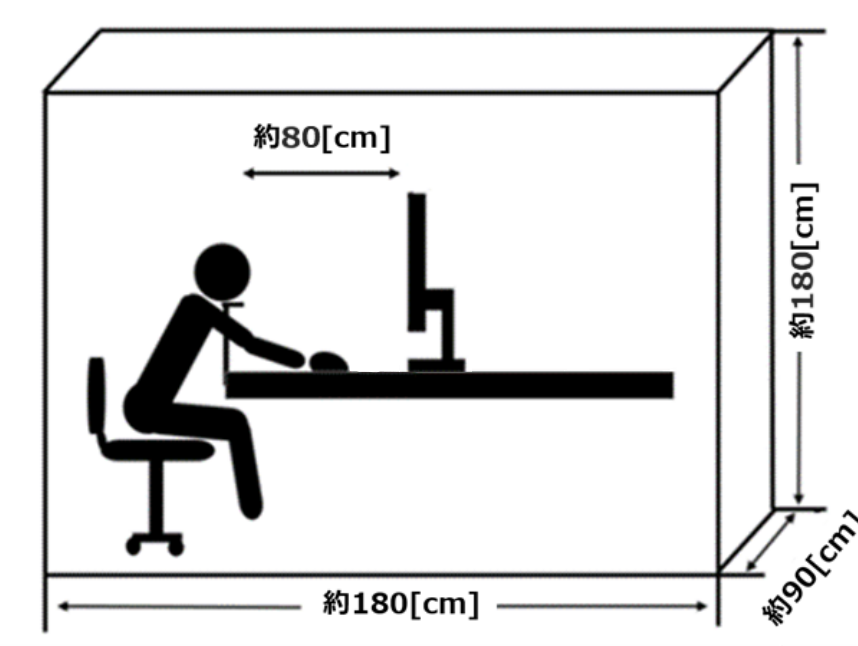
\includegraphics[width=10.0cm]{./img/darkroom_p.png}
                \caption{実験環境概略図}
                \label{darkroom}
            \end{figure}

            図\ref{darkroom}に実験環境の概略図を示す.
            暗幕で覆われた簡易的な暗室内に刺激呈示用液晶ディスプレイ (EIZO社,解像度 1920 ピクセル✕ 1200 ピクセル,リフレッシュレート 60 Hz) を設置し実験を行った.
            また,刺激の輝度と色度を正確に投影するために分光反射輝度計 (Cambridge Research Systems 社 SpectroCAL) によりモニタの分光分布を,色彩輝度計 (Cambridge Research Systems 社 ColorCAL2) によりモニタのガンマ特性を測定した.
            これにより,所望のCIE $XYZ$三刺激値をモニタに呈示することが可能となった.
            
            実験はすべてPC ( DELL 社 Vostro 13 5000, OS: Ubuntu 18.04.3 LTS) で統制され,MathWorks MATLAB と Psychtoolbox3\cite{Psychtoolbox} を用いてプログラムを作成・実行することでディスプレイの刺激呈示と被験者応答を管理した.
            実験中,被験者の頭部はディスプレイから 80 cm の距離に顎台により固定され,両眼自然視でディスプレイを観察した.
            被験者はトラックボールマウスを使用して応答した.

        \subsection{実験刺激}

            \begin{figure}[h]
                \centering
                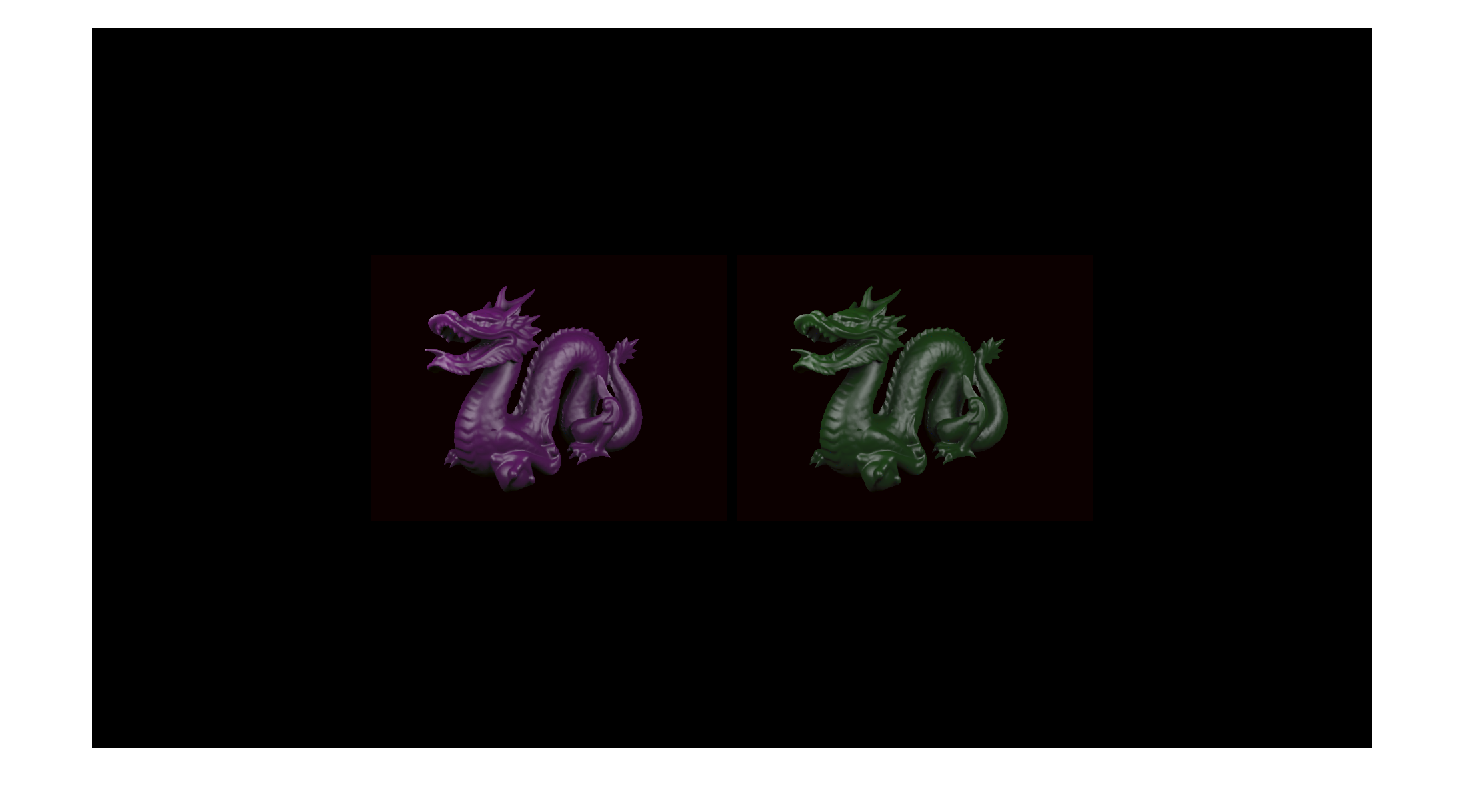
\includegraphics[width=14.0cm]{./img/ex1_stimuli.png}
                \caption{実験刺激の例}
                \label{ex1_stimuli}
            \end{figure}

            図\ref{ex1_stimuli}に実験1で使用する刺激を示す.
            刺激は黒背景上の中心部分の縦 6.42 deg, 横 17.35 deg の範囲の左右に呈示される二枚のコンピュータグラフィックス画像であった.
            これらの画像はモニタ中央を挟んで対称な位置に呈示された.
            また,各画像はコンピュータグラフィックスソフトウェアを用いたレンダリングと,MATLAB上での簡易的な画像処理を用いた着色の二つの工程を経て作られた.
            以下に,これらの工程の詳細を記す.

            \subsubsection{レンダリング}

                実験に用いた刺激の元となる無彩色刺激は RenderToolbox4 によって,レンダラーを Mitsuba\cite{Mitsuba} として作成された.
                この際の照明環境はCIE標準光源D65であり,物体の分光反射特性は全波長にわたり同じ値であった.
                物体形状として,Stanford Dragon と Stanford Bunny \cite{StanfordModels} の2種類を使用し,照明環境も含めた環境のジオメトリはBlender 2.79により設定した.
                一方,表面反射特性は RenderToolbox4 と Mitsuba により設定し,その反射モデルとして Ward モデル\cite{Ward}を用いた.
                この際,拡散反射成分と鏡面反射成分の色度を別々に操作するため,これらの反射成分は独立にレンダリングした.
                このレンダリングにおけるパラメータを表\ref{render_param}に示す.

                \begin{table}[h]
                    \centering
                    \caption{レンダリング時のパラメータ}
                    \begin{tabular}{|l||c|c|c|} \hline
                                            & SpecularReflectance & DiffuseReflectance & Roughness \\ \hline \hline
                        拡散反射成分           & 0                   & 0.1                & 0.2 \\ \hline
                        鏡面反射成分           & 0.9                 & 0                  & 0.2 \\ \hline
                    \end{tabular}
                    \label{render_param}
                \end{table}
            
            \subsubsection{色度の付与}

                レンダリングされた画像は上述したとおりD65の色度を持つ画像であったが,その画像に対して色条件を設定するために色度を付与した.
                その方法はSD着色とD着色の2種類であった.
                SD着色では,拡散反射成分と鏡面反射成分の両方に同じ色度を設定し,それらのCIE $XYZ$値を加算して作成した.
                D着色では,拡散反射成分にのみ色度を付与し,$XYZ$値を加算して作成した.
                この着色処理において,Mitsubaによってレンダリングされた画像のXYZ三刺激値を $u^{\prime}v^{\prime}Y$ 色空間に変換し, $u^{\prime}v^{\prime}$ 色度図上で行われた.
                その色度は全部で9種類である.
                そのうち1種類はD65の色度であり,これを白色点とする.
                その他の8種類の色度は,白色点を中心とし,$u^{\prime}v^{\prime}$ 色度図上の0°から45°間隔となる8方向にある色度であった.
                本論文では,これらの9色度をそれぞれgray, red, orange, yellow, green, blue-green, cyan, blue, magentaと呼ぶことにする.

                レンダリングされた画像は非常に高輝度な領域を含む画像であった.
                モニタが表示可能な色域は輝度によって異なり,特にモニタが表示できる最大・最小輝度付近における $u^{\prime}v^{\prime}$ 色度図の領域は非常に小さい.
                すなわち,この画像に対して着色処理を行った場合,高輝度になりやすい鏡面反射成分に十分な彩度の色度を付与することができない.
                このため,線形トーンマッピングによって画像の最高輝度を下げた.
                この時のトーンマッピング前後の最高輝度を表\ref{tonemap}に示す.

                \begin{table}[h]
                    \centering
                    \caption{トーンマップ前後のレンダリングされた画像の最高輝度}
                    \begin{tabular}{|l||c|c|} \hline
                                               & Dragon              & Bunny              \\ \hline \hline
                        トーンマップ前         & 714.1861            & 680.6588           \\ \hline
                        トーンマップ後         & 43.4937             & 43.6503            \\ \hline
                    \end{tabular}
                    \label{tonemap}
                \end{table}

                また,モニタが表示可能な色域は色相によっても異なる.レンダリングされた画像にモニタの色域外の色度を付与しないように,画像の輝度を対数尺度を用いて200段階に標本化し,そのそれぞれの輝度に対して9種類の色度の白色点から最大距離となる点を計測した.

                [未完成]

                
            以上の工程によって得られた全刺激画像を図\ref{ex1_stimuli_d}と図\ref{ex1_stimuli_b}に示す.

            \begin{figure}[h]
                \centering
                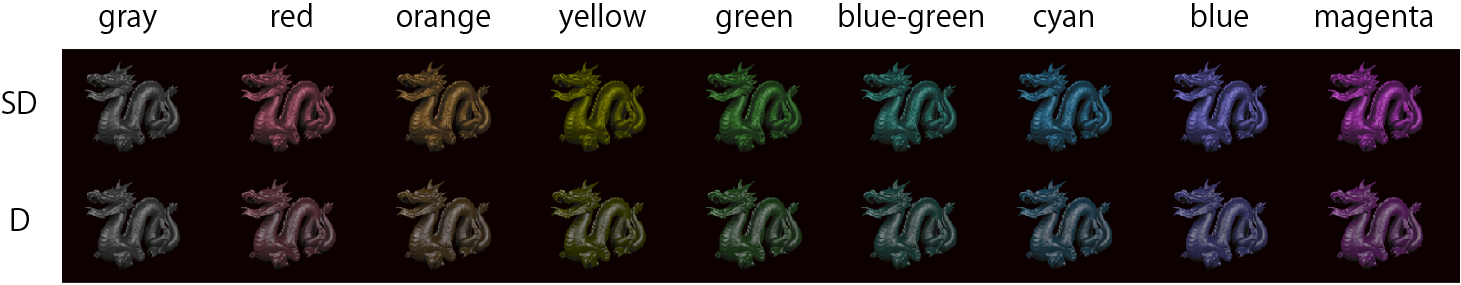
\includegraphics[width=14.0cm]{./img/ex1_stimuli_d_p.png}
                \caption{dragon形状の刺激画像}
                \label{ex1_stimuli_d}
            \end{figure}

            \begin{figure}[h]
                \centering
                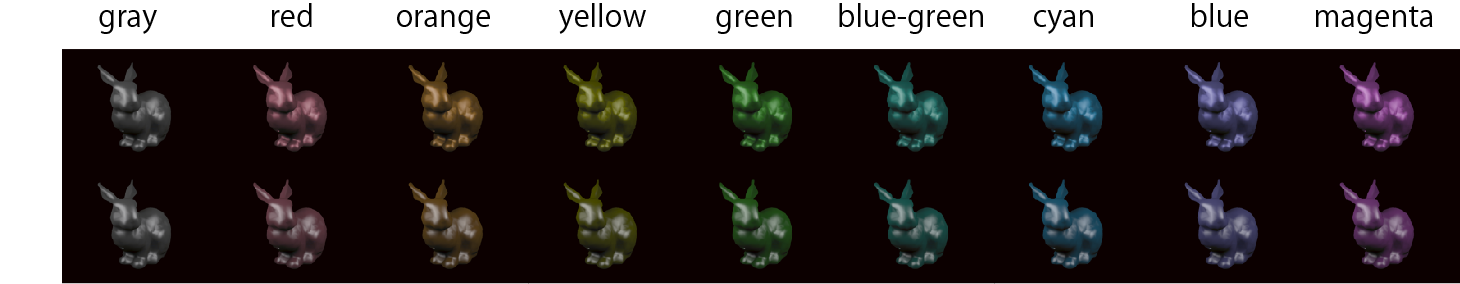
\includegraphics[width=14.0cm]{./img/ex1_stimuli_b_p.png}
                \caption{bunny形状の刺激画像}
                \label{ex1_stimuli_b}
            \end{figure}

        \subsection{実験手続き}

            \begin{figure}[h]
                \centering
                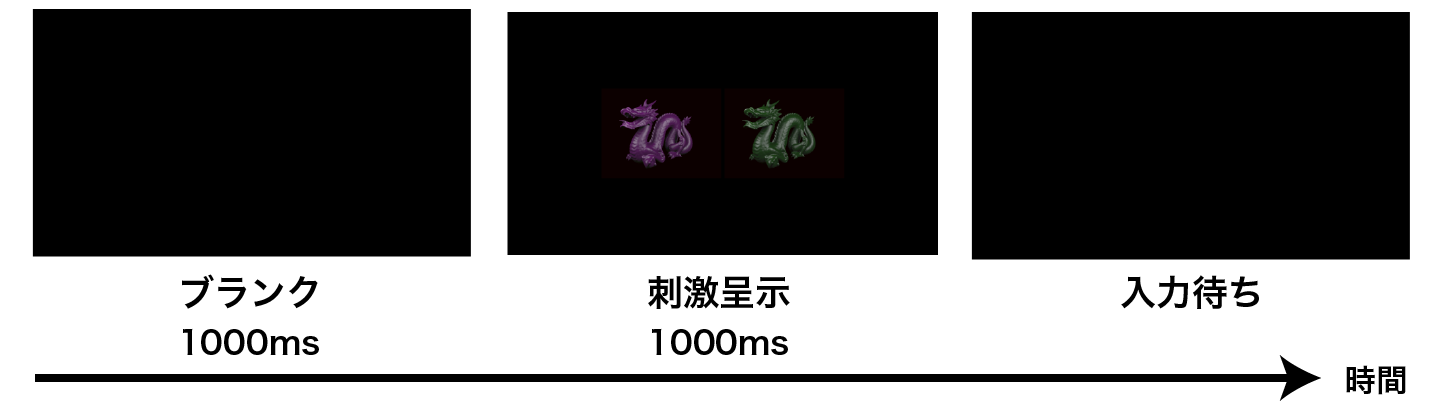
\includegraphics[width=14.0cm]{./img/ex1_procedure.png}
                \caption{1試行の流れ}
                \label{ex1_procedure}
            \end{figure}

            実験1はサーストンの一対比較法を用いて行われた.
            実験1の1試行の流れを図\ref{ex1_procedure}に示す.各試行はまず黒背景のみからなるブランク画面の1000msの呈示から始まる.
            その後,刺激対が1000msの間呈示され,さらに,色順応を避けるために黒背景のみからなる入力待ち画面に移行した.
            刺激対の呈示中または入力待ち画面で,被験者は右画像と左画像のうちどちらからより光沢感を強く知覚するかを,マウスの左クリックまたは右クリックにより応答した.
            このとき次の試行のブランク画面に移行した.

            各セッションは 2 着色条件 $\times$ 物体形状 2 種類 $\times$ 色の組み合わせ 36 通り = 144 試行からなる.
            各被験者は全体で4セッションの実験を行った.
            各セッションの 144 試行で使われる刺激対は全てランダムな順序で選ばれた.
            1セッションに要する時間はおよそ8分であり,2セッション目と3セッション目の間に一度だけ休憩をとった.



    \section{実験結果}
        \subsection{解析方法}
            被験者の応答結果から得られた勝敗表から,サーストンの一対比較法を用いて選好尺度値を算出した.
            次に,算出された選好尺度値を初期値とし,最尤法を用いて再び選好尺度値を算出した.
            この選好尺度値は光沢感の知覚量の指標となる.
            

        \newpage
        \subsection{各色度の刺激に対する選好尺度値}
            
            \begin{figure}[h]
                \centering
                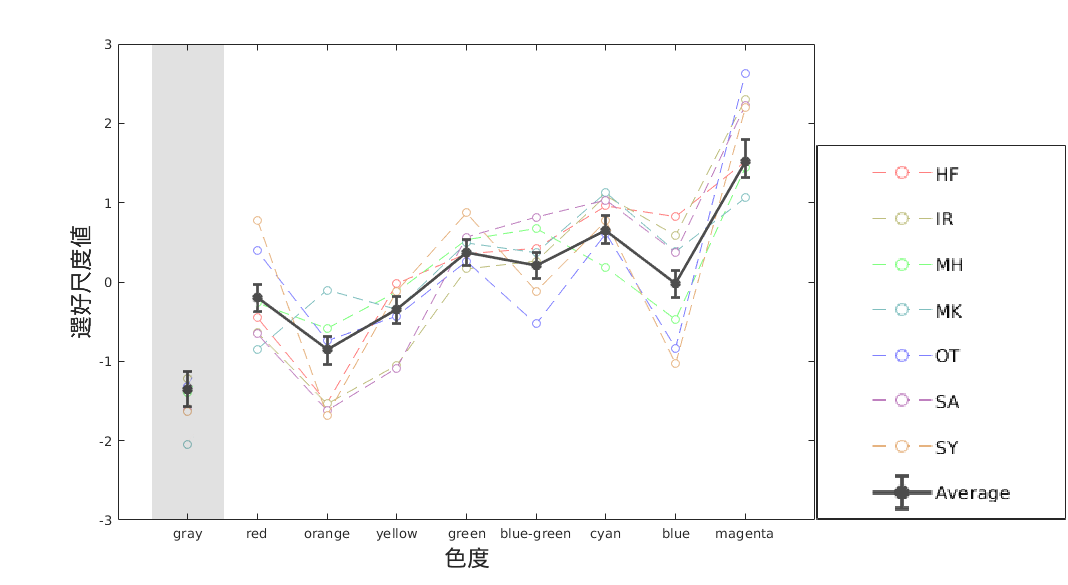
\includegraphics[width=15.0cm]{./img/ex1_res_DSD_p.png}
                \caption{Dragon形状のSD条件における選好尺度値}
                \label{ex1_DSD}
            \end{figure}

            \begin{figure}[h]
                \centering
                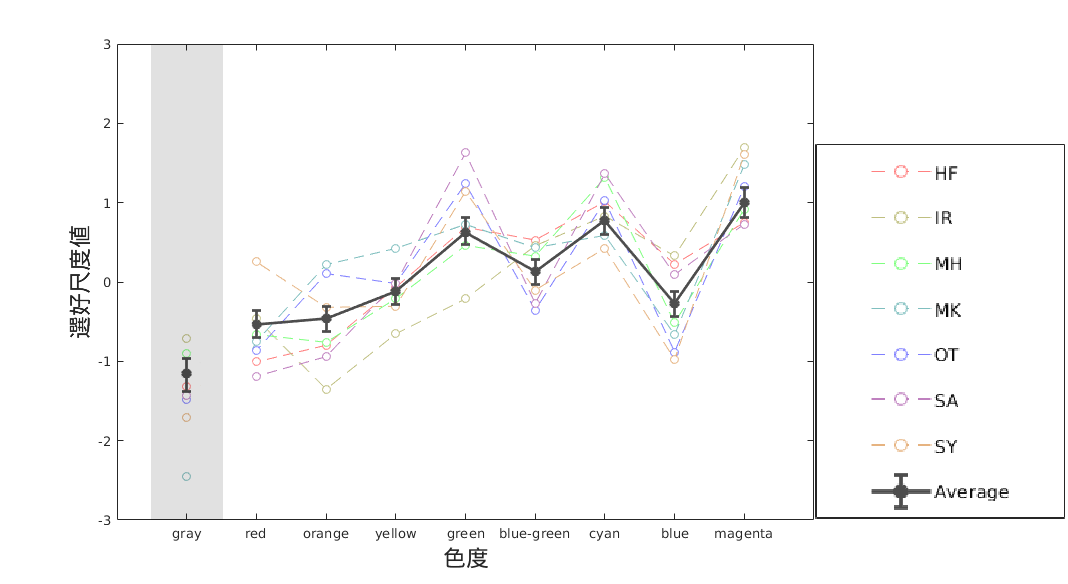
\includegraphics[width=15.0cm]{./img/ex1_res_BSD_p.png}
                \caption{Bunny形状のSD条件における選好尺度値}
                \label{ex1_BSD}
            \end{figure}
            
            \newpage
            \begin{figure}[h]
                \centering
                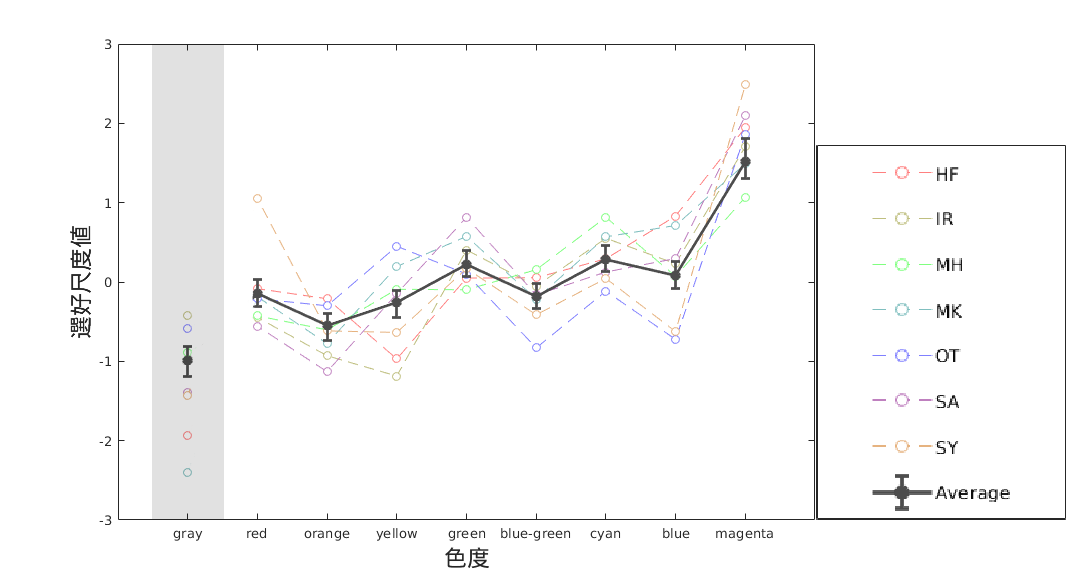
\includegraphics[width=15.0cm]{./img/ex1_res_DD_p.png}
                \caption{Dragon形状のD条件における選好尺度値}
                \label{ex1_DD}
            \end{figure}

            \begin{figure}[h]
                \centering
                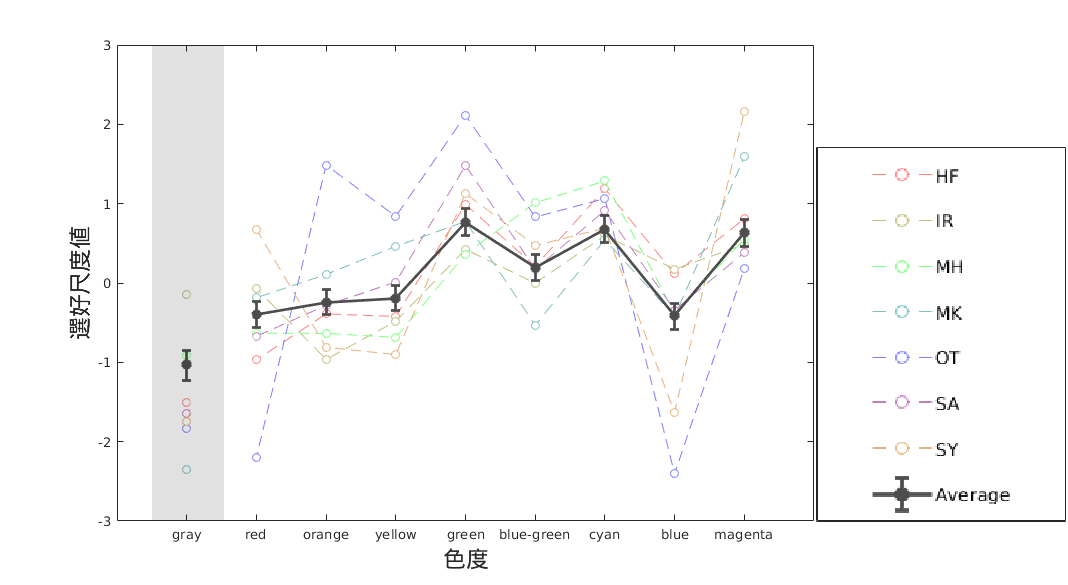
\includegraphics[width=15.0cm]{./img/ex1_res_BD_p.png}
                \caption{Bunny形状のD条件における選好尺度値}
                \label{ex1_BD}
            \end{figure}

            図\ref{ex1_DSD}から図\ref{ex1_BD}に各被験者と被験者間平均の選好尺度値を示す.
            縦軸は選好尺度値,横軸は色度の種類を表す.
            これらの統計学的仮説検定はリサンプリング回数1000回のノンパラメトリックブートストラップ検定により行われた.
            各図中の黒線のエラーバーはブートストラップ法による95\%信頼区間を表す.

            物体形状や着色条件に関わらず,すべての条件において色度による光沢感に違いがあった.
            特にBunny形状のD条件を除いてmagentaの光沢感が極めて高く,次いでgreen,cyanの光沢感が高いという結果となった.
            また,全ての形状と条件において有彩色の光沢感は無彩色の光沢感に比べて大きかった.
            Bunny形状のD条件では,他の3条件と比べてblueとmagentaの光沢感が比較的小さい値であったが,全体的に見てSD,D条件間では大きな傾向の違いは見られなかった.

    \section{考察}

        本実験の作業仮説が正しければ,SD条件とD条件の刺激間では明るさ感のコントラストが異なるために色度ごとの光沢感の傾向が異なるはずである.
        しかし,実験1の結果より,SD条件とD条件の応答の傾向について明確な傾向を見出すことができなかった.
        すなわち,光沢感が拡散反射と鏡面反射の知覚的な明るさのコントラストによって主に決まっているという訳ではないと言える.

        ここで,orangeとyellowの光沢感が比較的小さく,magentaの光沢感が極端に大きい点に着目する.
        これはH-K効果による明るさ感増幅の傾向の特徴と一致する.
        すなわち,刺激全体を通して感じられる明るさ感が光沢感に寄与しているという可能性が考えられる.

        刺激全体の明るさ感の効果量を測定するためには,本実験で用いた刺激の色度のH-K効果を調べる必要がある.
        このため,次章では本実験で用いた刺激の平均色のパッチを用いて実験を行う.

    \newpage